\chapter{Xây dựng phiên bản thử nghiệm}
\section{Công nghệ sử dụng}
Để hiện thực hệ thống, nhóm quyết định sử dụng các công nghệ sau:
\begin{itemize}
    \item ReactJS: Hiện thực UI, frontend.
    \item Java Springboot: Hiện thực microservice, backend.
    \item PostgresSQL: Hệ cơ sở dữ liệu lưu trữ thông tin.
    \item Kubernetes: Deploy các microservice.
    \item Minikube: Chạy Kubernetes cluster trên local.
    \item Terraform: Khởi tạo 
\end{itemize}

\section{Giới hạn phạm vi}
\subsection{Về mặt nghiệp vụ}
\noindent Sau khi bàn bạc, nhóm đi tới thống nhất là sẽ hiện thực phần Trang chủ (Home page - Catalog), vì đó là thành phần mà người dùng sẽ gặp đầu tiên khi bắt đầu truy cập vào hệ thống.
\subsection{Về mặt thành phần hệ thống}
\noindent Sau khi cân nhắc kỹ lưỡng, để đảm bảo cho phiên bản demo thể hiện được trọn vẹn và đầy đủ nhất các tính chất cốt lõi của hệ thống, nhóm đã giới hạn phạm vi hiện thực của hệ thống xuống còn các thành phần như sau:
\begin{itemize}
    \item Frontend: Trang chủ - Catalog, thể hiện danh sách các mặt hàng đang được bày bán 
    \item Backend: Catalog service, cung cấp API danh sách sản phẩm.
    \item Minikube cluster: Cung cấp môi trường Kubernetes cluster local trên máy tính cá nhân.
    \item Deployment: Thành phần cơ bản nhất của hệ thống, dùng để quản lý trực tiếp các pod.
    \item Service: Một lớp ảo hóa để các thành phần khác có thể truy cập tới các pod.
    \item Ingress: Đóng vai trò như reverse proxy, cung cấp API gateway để kết nối từ bên ngoài cluster tới service.
    \item Horizontal Pod Autoscaler: Dùng để tăng hoặc giảm số pod một cách tự động, dựa trên các thông số (metrics) của chính các pod đó.
\end{itemize}
\section{Nội dung hiện thực}
\subsection{Hiện thực frontend và backend}
\noindent Sau khi có một ứng dụng hoàn chỉnh, có thể hiển thị được thông tin mặt hàng, ta đóng gói nó thành Docker image và đẩy lên Docker Hub.\\[0.5cm]
Dockerfile của frontend có nội dung như sau:
\begin{lstlisting}[language=docker]
# Use an official Node runtime as a parent image
FROM node:18 AS builder

# Set the working directory in the container
WORKDIR /app

# Copy package.json and package-lock.json to the container
COPY package.json ./

# Install dependencies
RUN npm install

# Copy the rest of the application code to the container
COPY . .

# Build the Vite React application
RUN npm run build

# Use an official Nginx runtime as a parent image
FROM nginx:alpine

# Copy the build output from the builder stage to the nginx web root
COPY --from=builder /app/dist /usr/share/nginx/html

# Expose port 80
EXPOSE 80
\end{lstlisting}

Dockerfile của backend có nội dung như sau:

\begin{lstlisting}[language=docker]
# Use an official OpenJDK runtime as a base image with Java 17
FROM eclipse-temurin:17-jdk-alpine

# Set the working directory to /app
WORKDIR /app

# Copy the current directory contents into the container at /app
COPY . /app

# Build the Spring Boot application
RUN ./mvnw package -DskipTests

# Expose the port that your Spring Boot application will run on
EXPOSE 80

# Define the command to run your application
CMD ["java", "-jar", "target/catalog-0.0.1-SNAPSHOT.jar"]
\end{lstlisting}

\subsection{Hiện thực Deployment và Service}
\noindent Ta sử dụng terraform để khởi tạo các service trên, tương ứng với mỗi microservice frontend và backend.
\subsubsection{Với frontend}
\noindent Với frontend, khi được đưa lên production, service sẽ được build thành định dạng html, css truyền thống, đi kèm với file javascript chứa logic, và được cung cấp bởi Nginx server, do đó mặc định port sẽ là 80 (HTTP).
\begin{lstlisting}[language=terraform]
resource "kubernetes_deployment" "catalog-fe-deploy" {
  metadata {
    name = "catalog-fe-deploy"
    labels = { app = "catalog-fe", tier = "frontend" }
  }
  spec {
    replicas = 1
    selector {
      match_labels = { app = "catalog-fe-pod", tier = "frontend" }
    }
    template {
      metadata {
        name = "catalog-fe-pod"
        labels = { app = "catalog-fe-pod", tier = "frontend"}
      }
      spec {
        container {
          name = "catalog-fe"
          image = "hoanganhleboy/catalog-fe:latest"
          port { container_port = 80 }
          env {
            name = "CONTENT"
            value = "This is the string from k8s"
          }
          image_pull_policy = "Always"
        }
      }
    }
  }
}

resource "kubernetes_service" "catalog-fe-service" {
  metadata {
    name = "catalog-fe-service"
    labels = { app = "catalog-fe-service", tier = "frontend" }
  }
  spec {
    selector = { app = "catalog-fe-pod", tier = "frontend"}
    port {
      protocol = "TCP"
      port = 80
      target_port = 80
    }
    type = "NodePort"
  }
}
\end{lstlisting} 
\subsubsection{Với backend}
\noindent Catalog microservice sau khi được build thành image sẽ được chạy từ file .jar, thông qua JVM.
\begin{lstlisting}[language=terraform]
resource "kubernetes_deployment" "catalog-ms-deploy" {
  metadata {
    name = "catalog-ms-deploy"
    labels = { app = "catalog-ms", tier = "backend" }
  }
  spec {
    replicas = 1
    selector {
      match_labels = { app = "catalog-ms-pod", tier = "backend" }
    }
    template {
      metadata {
        name = "catalog-ms-pod"
        labels = { app = "catalog-ms-pod", tier = "backend"}
      }
      spec {
        container {
          name = "catalog-ms"
          image = "hoanganhleboy/catalog-ms"
          port { container_port = 8090 } // This port the same with port in the code.
          resources {
            requests = {
              cpu = "256m"
              memory = "128Mi"
            }
            limits = {
              cpu = "256m"
              memory = "128Mi"
            }
          }
        }
      }
    }
  }
}

resource "kubernetes_service" "catalog-ms-service" {
  metadata {
    name = "catalog-ms-service"
    labels = { app = "catalog-ms-service", tier = "backend" }
  }
  spec {
    selector = { app = "catalog-ms-pod", tier = "backend"}
    port {
      protocol = "TCP"
      port = 8090 // port expose to outside
      target_port = 80 // This port the same with port in the code.
    }
    type = "NodePort"
  }
}
\end{lstlisting}
\section{Hiện thực Ingress}
\noindent Ingress hiện tại đóng vai trò là reverse proxy, expose các Kubernetes service ra bên ngoài cluster.
\begin{lstlisting}[language=yaml]
apiVersion: networking.k8s.io/v1
kind: Ingress
metadata:
  name: example-ingress
  annotations:
    nginx.ingress.kubernetes.io/enable-directory-listing: "true"
    nginx.ingress.kubernetes.io/rewrite-target: /$2
spec:
  rules:
    - http:
        paths:
          - pathType: Prefix
            path: /backend(/|$)(.*)
            backend:
              service:
                name: catalog-ms-service
                port:
                  number: 80
          - pathType: Prefix
            path: /frontend/?(.*)
            # path: /
            backend:
              service:
                name: catalog-fe-service
                port:
                  number: 80
---

\end{lstlisting}
\section{Hiện thực Horizontal Pod Autoscaler}
\noindent Horizontal Pod Autoscaler (HPA) được sử dụng để giúp deployment có thể scale lên và scale xuống số lượng pod tùy theo thông số nào đó của hệ thống. HPA được hiện thực như sau:
\begin{lstlisting}[language=yaml]
apiVersion: autoscaling/v2
kind: HorizontalPodAutoscaler
metadata:
  name: catalog-ms-hpa
spec:
  maxReplicas: 10
  metrics:
  - resource:
      name: cpu
      target:
        averageUtilization: 10
        type: Utilization
    type: Resource
  minReplicas: 1
  scaleTargetRef:
    apiVersion: apps/v1
    kind: Deployment
    name: catalog-ms-deploy
  behavior:
    scaleUp:
      selectPolicy: Max
      stabilizationWindowSeconds: 60
      policies:
      # number of pods that scale in a period of time
        - periodSeconds: 30
          type: Pods
          value: 4
    scaleDown:
      selectPolicy: Min
      stabilizationWindowSeconds: 60
      policies:
      # number of pods that scale in a period of time
        - periodSeconds: 30
          type: Pods
          value: 4
\end{lstlisting}
\section{Kiểm thử hệ thống}
\subsection{Thiết lập}
\noindent Sử dụng minikube, ta tạo một cluster với driver là docker (chạy trên nền docker), bằng câu lệnh \lstinline|minikube start --driver=docker|. Sau đó, ta cần kích hoạt 2 add on cần thiết cho ingress và HPA bằng 2 câu lệnh sau:
\begin{itemize}
  \item \lstinline|minikube addons enable ingress|
  \item \lstinline|minikube addons enable metrics-server|
\end{itemize}
Với addon ingress, ta có thể thiết lập và cấu hình ingress cho cluster. Addon metrics-server đóng vai trò cung cấp, theo dõi các thông số của pod (cpu, memory) nhằm phục vụ cho HPA.\\[0.5cm]
Sau đó, ta sẽ chạy cặp lệnh \lstinline|terraform init| để terraform tải và thiết lập sẵn các dependency cần thiết, và \lstinline|terraform apply --auto-approve| để khởi tạo các dịch vụ Kubernetes được viết bằng terraform.\\[0.5cm]
Với các dịch vụ được viết bằng yaml, ta cần chạy lệnh \lstinline|kubectl apply -f <file_name>| với \lstinline|<file_name>| là tên file config được viết bằng yaml.
\subsection{Kiểm tra tính sẵn sàng - availability}
\noindent Để kiếm tra tính sẵn sàng của hệ thống, ta sẽ thử xóa pod đi xem chuyện gì sẽ xảy ra.\\[0.5cm]
Đây là trạng thái ban đầu của các pod:
\begin{figure}[H]
  \begin{center}
  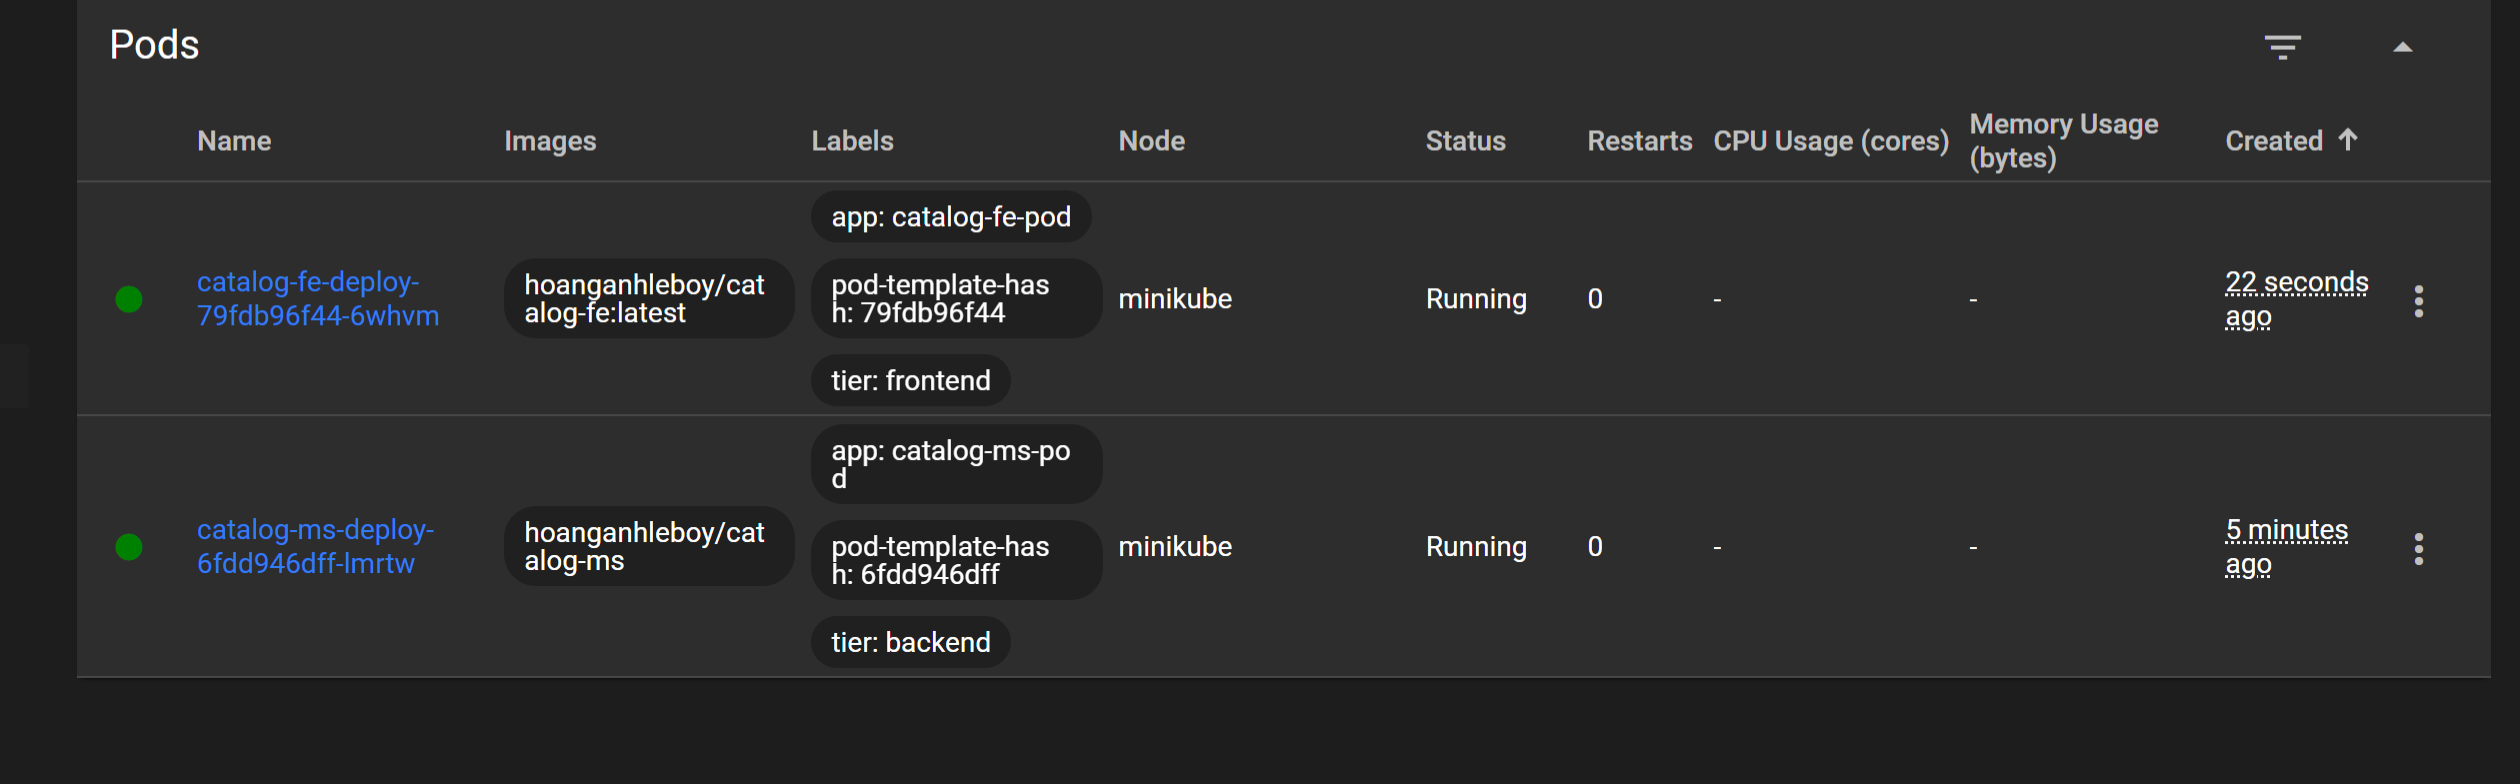
\includegraphics[scale=0.45]{images/hanh/pod_before_delete.png}
  \caption{Hình ảnh trước khi xóa pod}
  \end{center}
\end{figure}
Còn đây là hình ảnh sau khi vừa xóa:
\begin{figure}[H]
  \begin{center}
  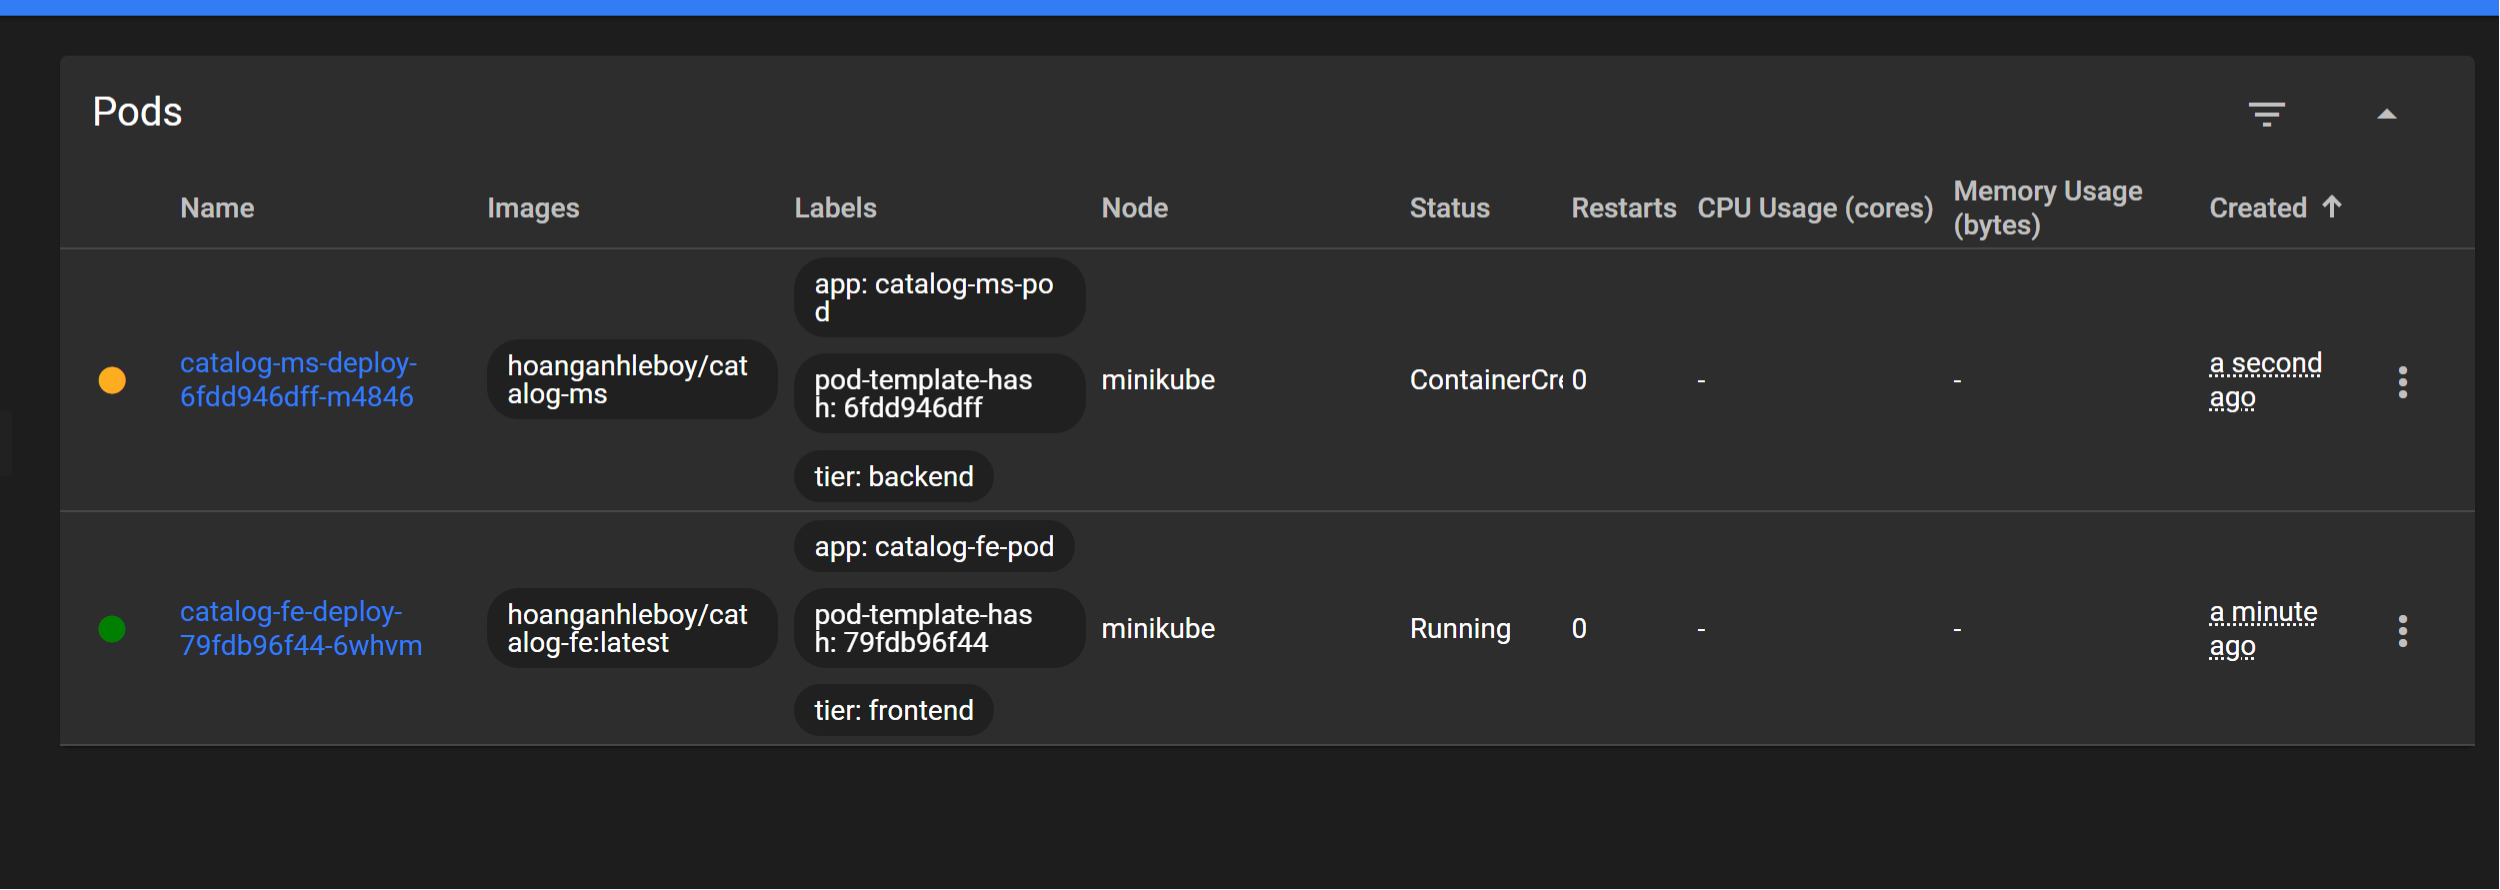
\includegraphics[scale=0.45]{images/hanh/pod_after_delete.png}
  \caption{Hình ảnh sau khi vừa xóa pod}
  \end{center}
\end{figure}
Như ta nhìn thấy trong hình 5.1 và 5.2, khi một pod vừa bị xóa, ngay lập tức một pod khác được khởi động ngay lập tức, thế chỗ cho pod vừa bị xóa. Như vậy, ta có thể kết luận rằng, khi triển khai hệ thống bằng Kubernetes, cụ thể là Deployment, tính sẵn sàng - availability của hệ thống được đảm bảo.
\subsection{Kiếm tra tính mở rộng - scalability}
\subsubsection{Manual scaling}
\noindent Tính mở rộng là việc hệ thống có thể tạo ra thêm nhiều bản sao của microservice, chạy song song với nhau nhằm đáp ứng được lượng request trên giây tương ứng của người dùng. Với Kubernetes, ta có thể dễ dàng scale up hay scale down hệ thống bằng tay thông qua việc điều chỉnh miền \lstinline|replicas| trong file config của Deployment.\\[0.5cm]
Ví dụ như hình 5.3 dưới đây, khi ta tăng số lượng pod của catalog-ms từ 1 lên 3
\begin{figure}[H]
  \begin{center}
    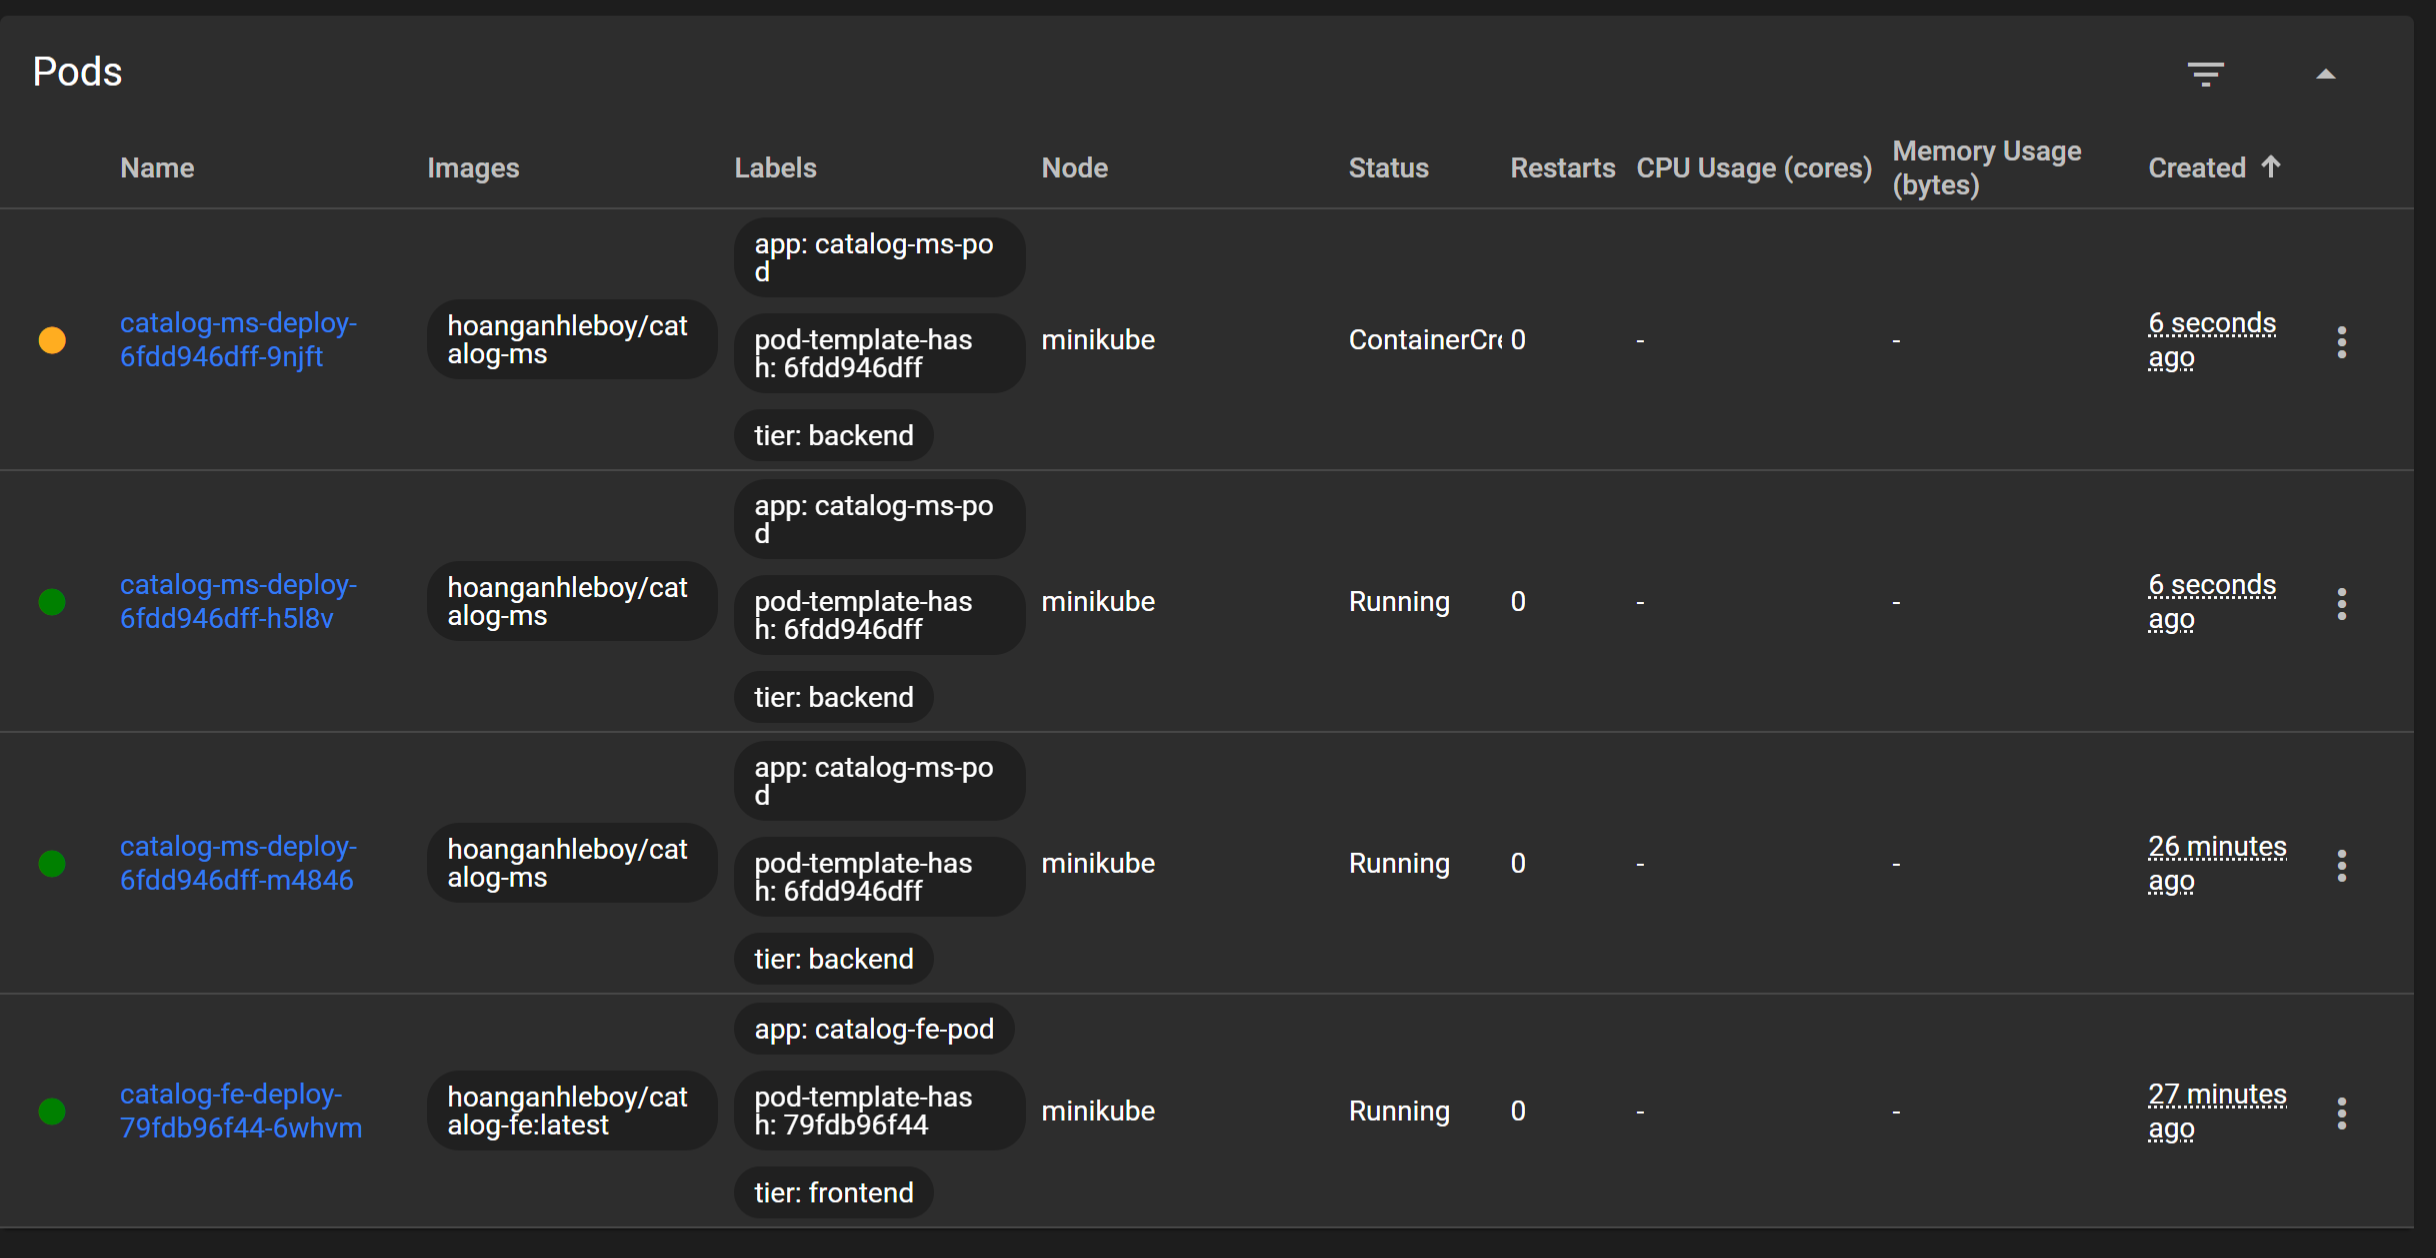
\includegraphics[scale=0.45]{images/hanh/catalog_ms_scale_up.png}
    \caption{Hình ảnh khi scale số pod từ 1 lên 3}
  \end{center}
\end{figure}
Ngay lập tức đã có thêm 2 pod mới được tạo ra như hình. Sau đó, khi ta giảm xuống 1 lại thì:
\begin{figure}[H]
  \begin{center}
    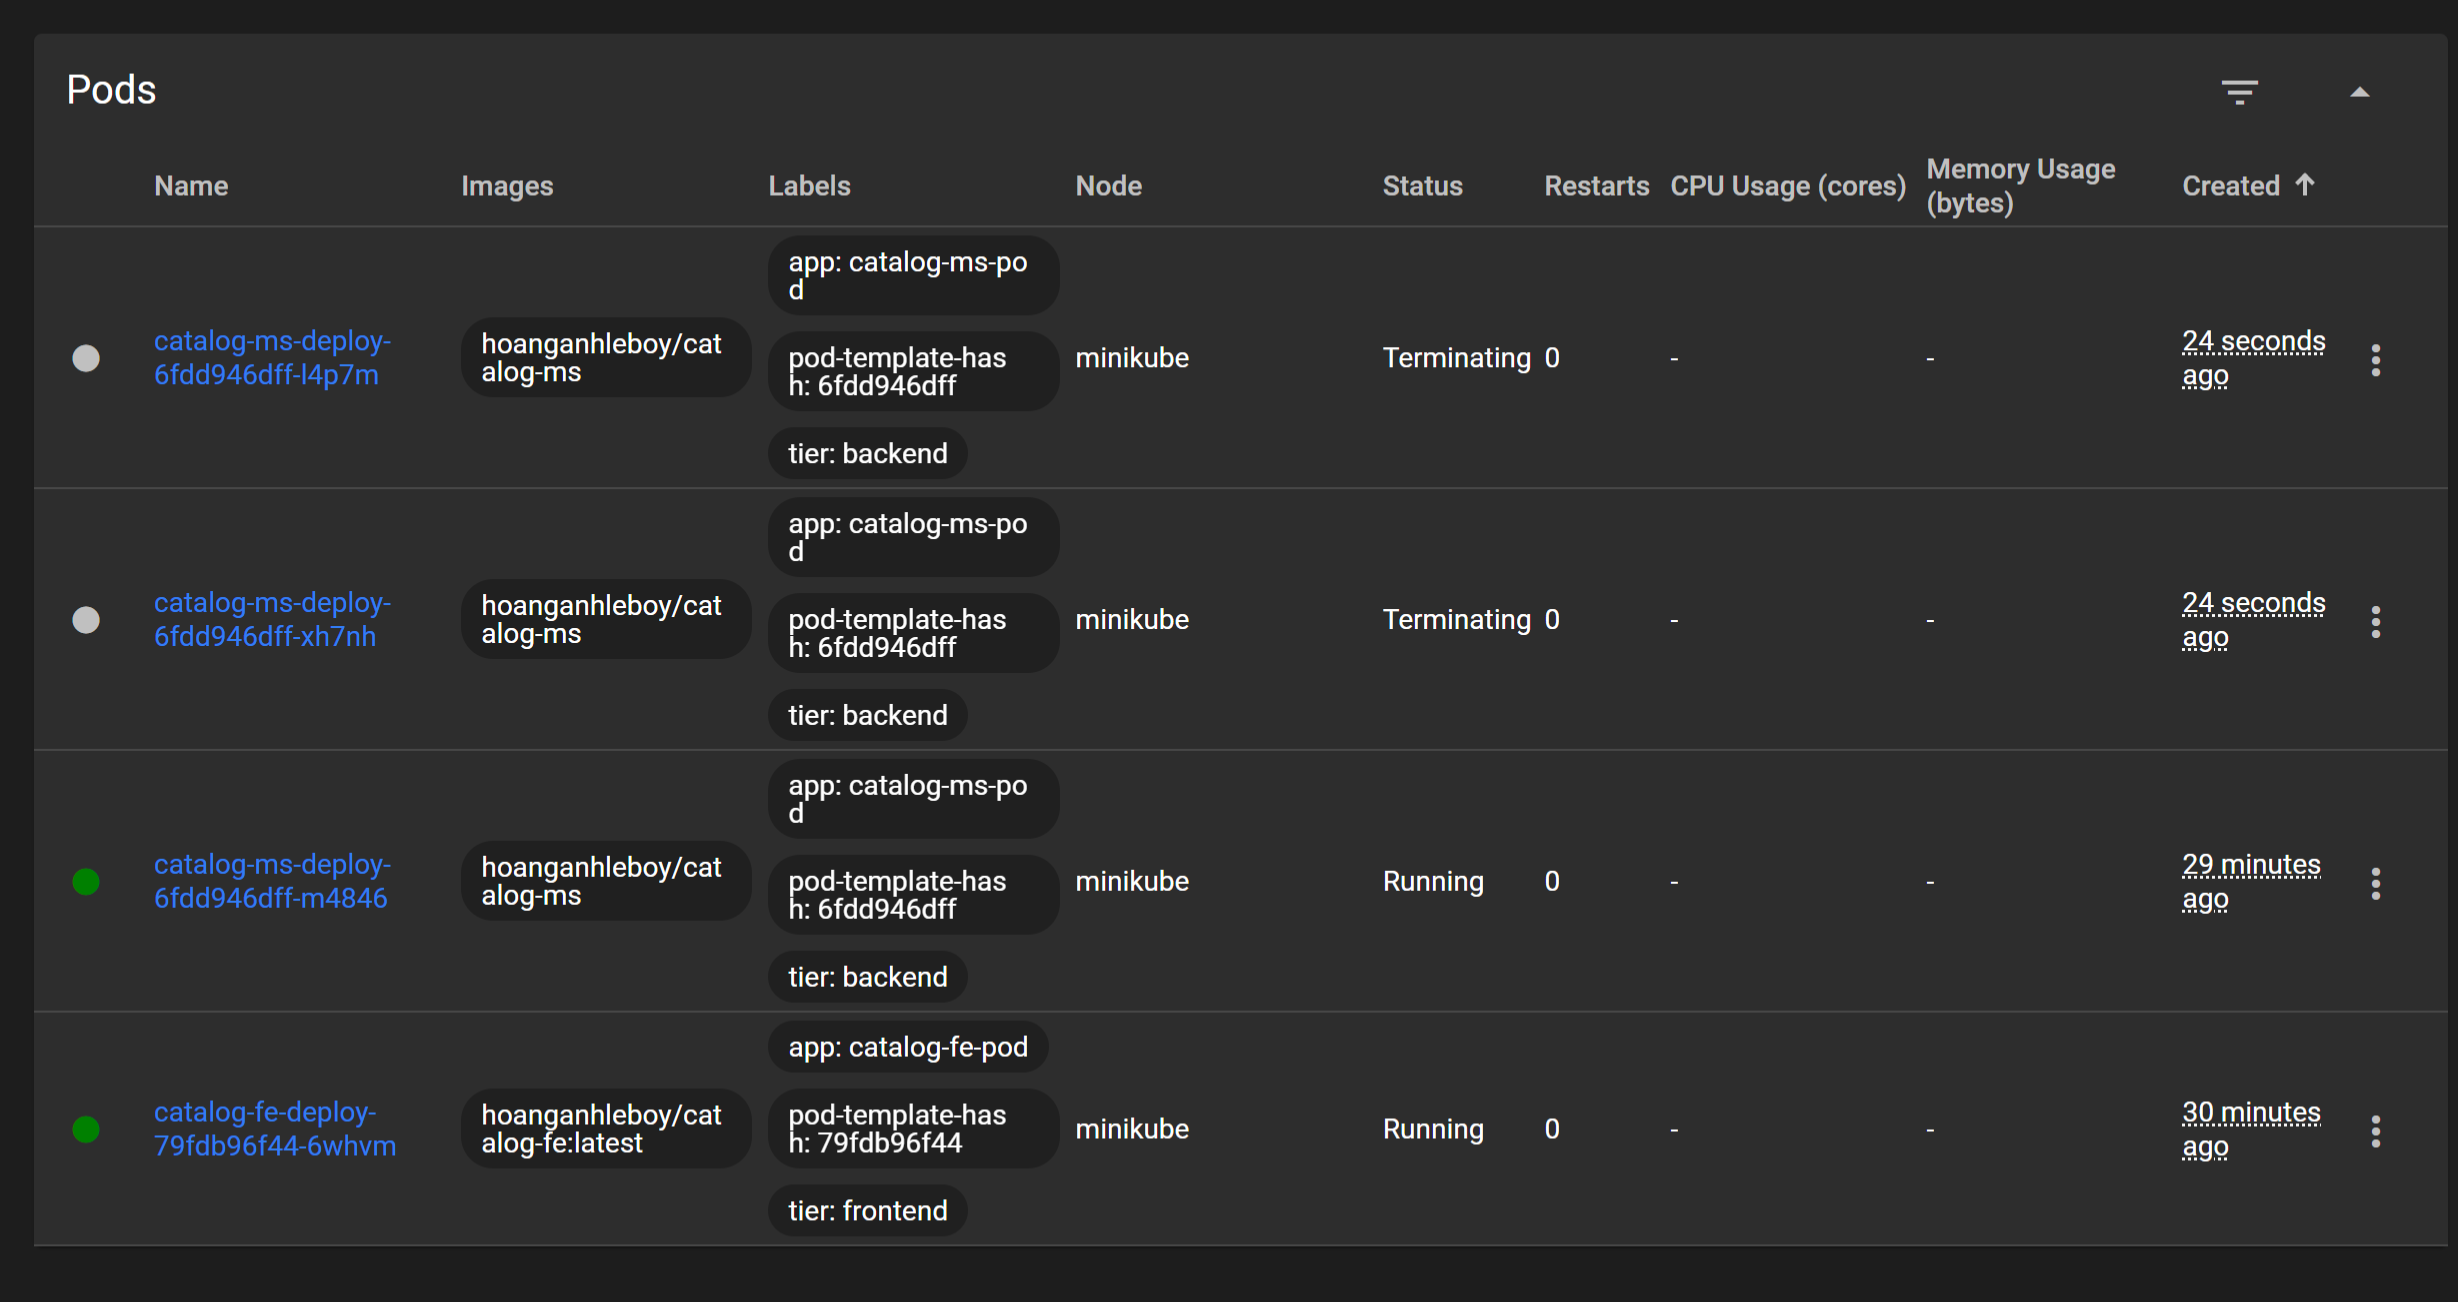
\includegraphics[scale=0.45]{images/hanh/catalog_ms_scale_down.png}
    \caption{Hình ảnh khi scale số pod từ 3 xuống 1}
  \end{center}
\end{figure}
Như hình 5.4, ta thấy ngay lập tức có 2 pod bị xóa đi để đảm bảo số lượng pod trong cluster về đúng số lượng quy định.

\subsubsection{Auto scaling}
Tuy nhiên, trên thực tế, việc scale thủ công như trên sẽ gây tiêu tốn tài nguyên về cả nhân lực và vật lực kha khá, do cần phải có sự can thiệp trực tiếp của con người, và cũng cần con người giám sát 24/24 để đảm bảo có thể điều chỉnh lượng pod phù hợp với nhu cầu lúc đó. Do đó, tốt hơn hết là ta nên thiết lập để Kubernetes có thể thực hiện việc đó một cách tự động thay cho chúng ta, và đó là khi ta cần dùng tới HPA - Horizontal Pod Autoscaler.\\[0.5cm]
Bài kiểm tra bao gồm các bước sau:
\begin{enumerate}
  \item Triển khai Deployment, Service, và HPA cho đối tượng muốn kiểm tra, ở đây là Catalog backend microservice.
  \item Khởi tạo một pod có chứa container được chạy từ image busybox, pod này sẽ cung cấp cho chúng ta môi trường linux shell. Ta sau đó viết 1 đoạn script tạo một vòng lặp vô hạn gọi tới API của Catalog backend microservice.
  \item Sử dụng câu lệnh \lstinline|kubectl get hpa --watch| để theo dõi trạng thái của HPA. Một thời gian sau, khi lượng pod đã được scale tới tối đa, ta tắt script để ngưng gọi API. 
  \item Lại đợi một khoảng thời gian, số pod đã được scale về mức tối thiểu. 
\end{enumerate}
\begin{figure}[H]
  \begin{center}
    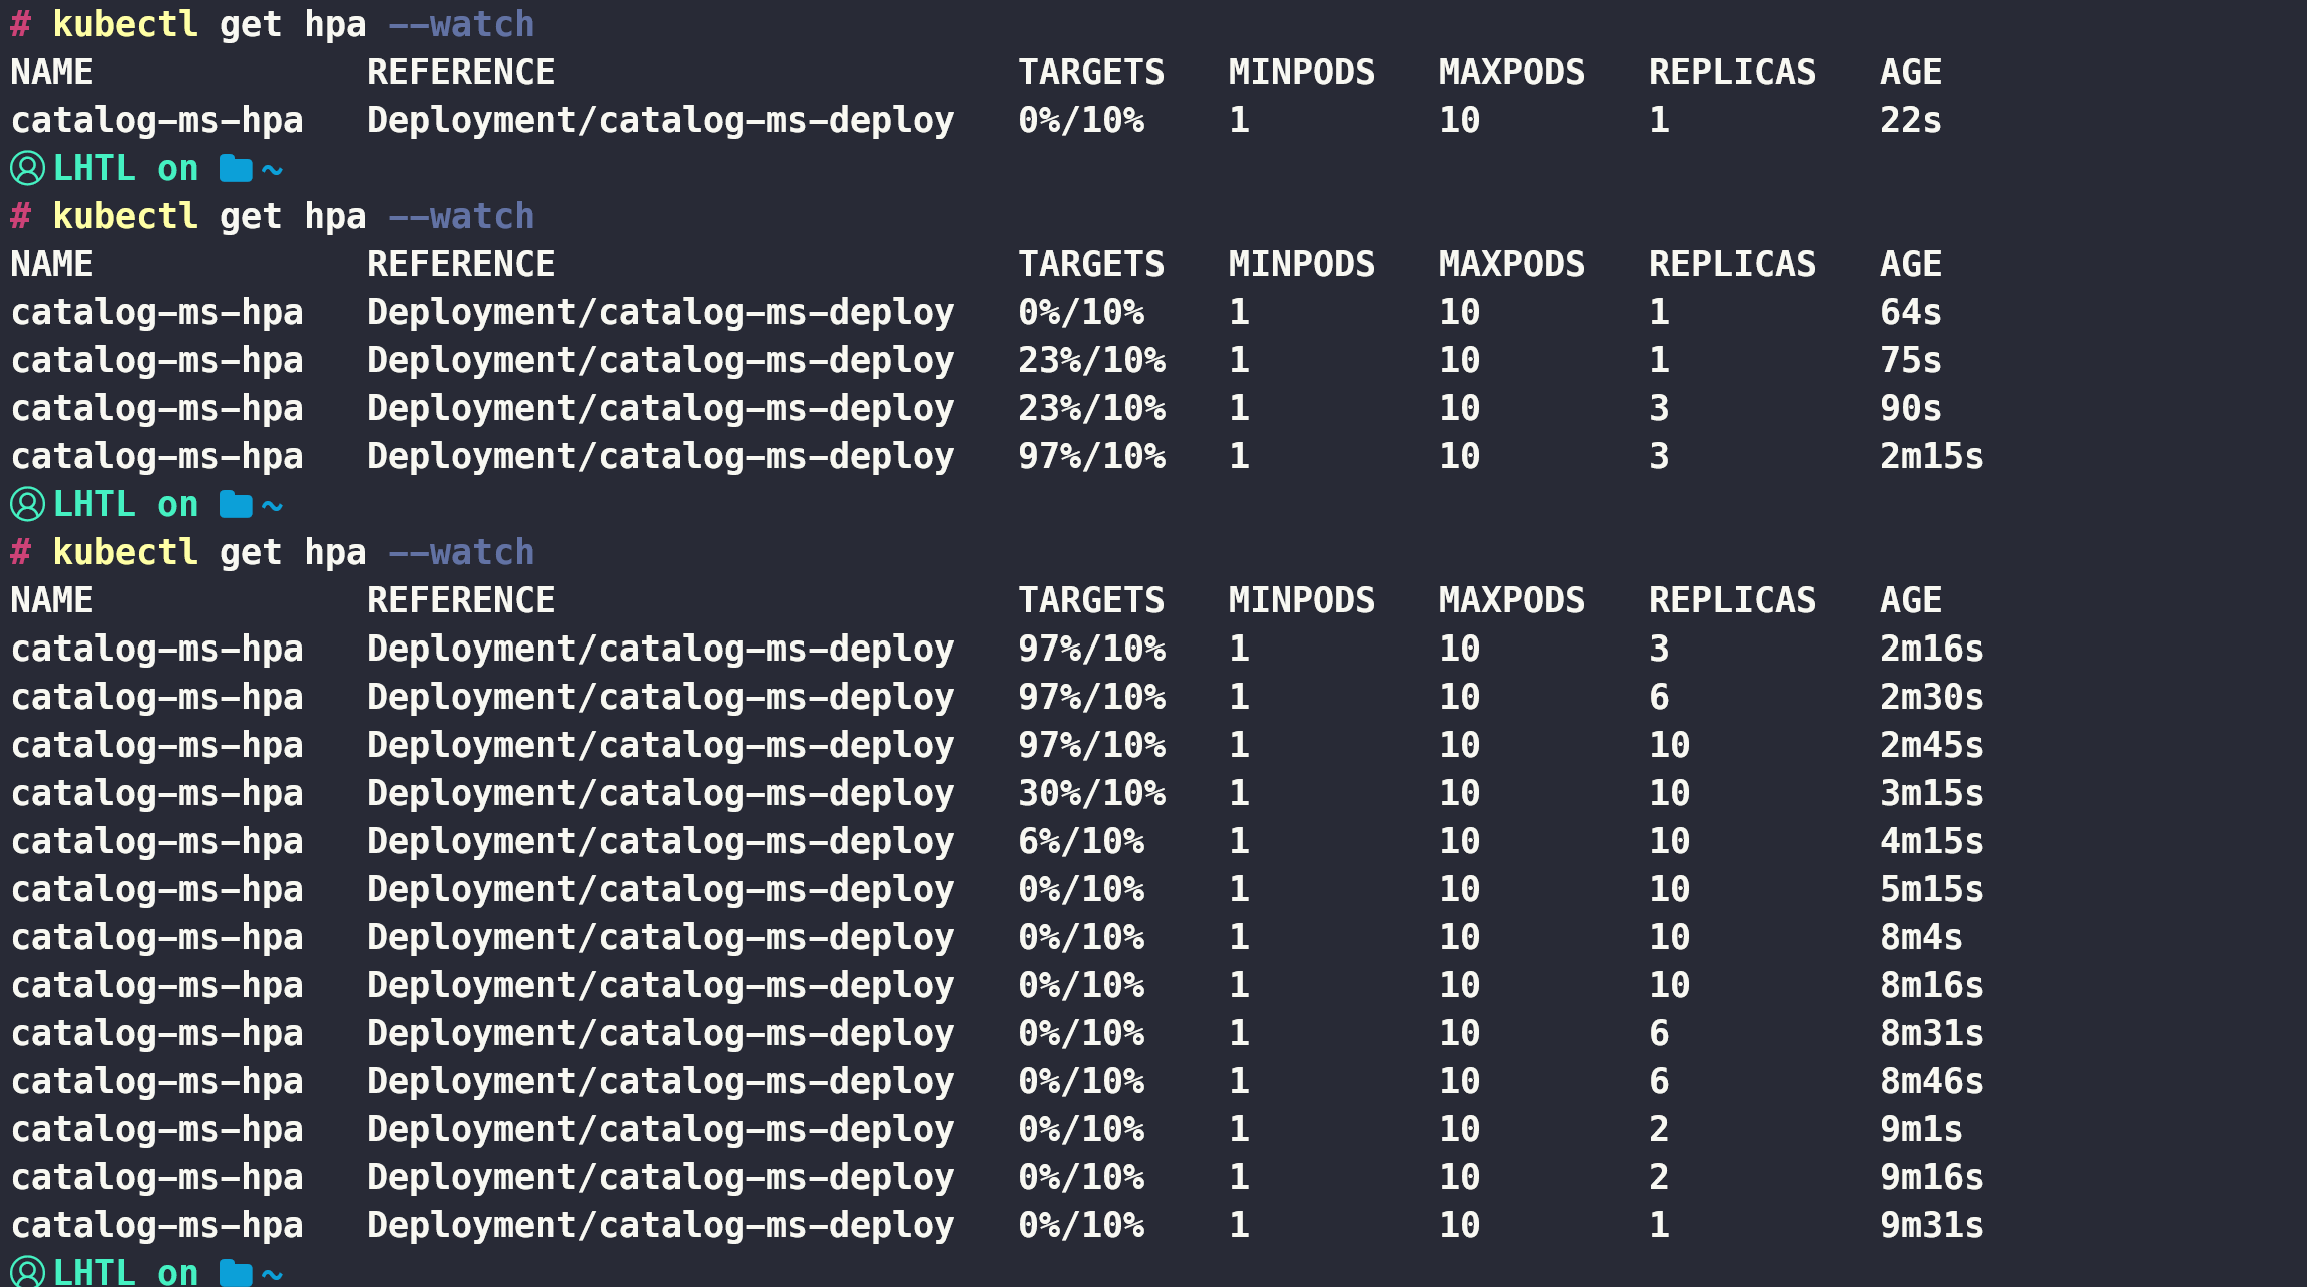
\includegraphics[scale=0.19]{images/hanh/HPA_CPU_scale.png}
    \caption{Kết quả cuộc thử nghiệm}
  \end{center}
\end{figure}
\noindent \textbf{Mô tả thí nghiệm:} Trong hình 5.5, ta có thể thấy khi bắt đầu gọi API liên tục tới Catalog backend server, thì CPU load bắt đầu tăng mạnh. Khi CPU load vượt ngưỡng 10\% thì HPA sẽ được kích hoạt để tăng số pod trong deployment lên, nhằm mục đích làm giảm PCU load xuống. Tuy nhiên, một thời gian ngắn sau vì CPU load tiếp tục vượt ngưỡng nên HPA lại tiếp tục được kích hoạt tiếp để tăng thêm số pod ở deployment. Việc này chỉ dừng lại cho đến khi số pod đã đạt ngưỡng tối đa cho phép, hoặc CPU load ổn định không tiếp tục vượt ngưỡng nữa thì thôi.\\[0.5cm]
Sau khi đã scale số pod lên đến mức tối đa là 10, ta terminate busybox đi để ngừng việc gửi request tới Catalog microservice. Lúc này CPU load giảm mạnh xuống còn 0\%. Sau một khoảng thời gian, HPA lại được kích hoạt để giảm số pod xuống. Khi giảm pod, nhận thấy CPU load vẫn tiếp tục dưới ngưỡng, HPA tiếp tục được kích hoạt để giảm tiếp số pod xuống, đến khi nào CPU load xấp xỉ với ngưỡng, hoặc khi đạt đến số pod tối thiểu, ở đây là 1 pod.